
%%%%%%%%%%%%%%%%%%%%%%%%%%%%%%%%%%%%%%%%%%%%%%%%%%%%%%%%%%%%
%%%%%%%%%%%%%%%%%%%%%%%%%%%%%%%%%%%%%%%%%%%%%%%%%%%%%%%%%%%%%
%
%  %%%%%%%  %    %  %%%%%%  %%%%%%  %%%%%%%  %%%%%%%  %%%%%
%  %        %    %  %    %  %     %    %     %        %    %
%  %        %    %  %%%%%%  %     %    %     %        %    %
%  %        %%%%%%  %    %  %%%%%%     %     %%%%%    %%%%%
%  %        %    %  %    %  %          %     %        %    %
%  %%%%%%%  %    %  %    %  %          %     %%%%%%%  %     %
%
%%%%%%%%%%%%%%%%%%%%%%%%%%%%%%%%%%%%%%%%%%%%%%%%%%%%%%%%%%%%%
%%%%%%%%%%%%%%%%%%%%%%%%%%%%%%%%%%%%%%%%%%%%%%%%%%%%%%%%%%%%%
\chapter{Graded Descriptions of the Derived Category}
\label{sec:graded}

\begin{quote}
{\em``Mathematics is the art of giving the same names to different things.''}
\begin{flushright} --- Henri Poincar\'e~\cite{poincare1908future} \end{flushright}
\end{quote}

In Chapter~\ref{sec:derived} we introduced the derived category of cellular sheaves. The fundamental objects there are chain complexes parametrized by a cell complex. However, the derived category takes a further step by identifying objects that are ``essentially the same'' when viewed through the lens of cohomology sheaves.

In Section~\ref{subsec:derived_vect} we understand this principle better by demonstrating the well known fact that the derived category of chain complexes of vector spaces (sheaves over a point) is equivalent to the graded category of vector spaces. Our proof follows the standard proof in~\cite{weibel} except we use the barcode method for chain complexes introduced in Example~\ref{ex:chaincomplex_bc} to visualize explicitly what is happening. Roughly speaking, the derived category of chain complexes allows us to remove the green bars in Figure~\ref{fig:bar_chain} as they ``graph'' the chain homotopy between the identity and the map that projects onto and then includes the red dots.

This sets us up for Section~\ref{subsec:derived_graded_cellsheaves}, which culminates in a proof that the derived category of cellular sheaves over a one-dimensional base space is equivalent to a graded category of sheaves. This should seem plausible because over each cell, a chain complex is equivalent to a graded vector space. Indeed, one could repeat the proof of Lemma~\ref{lem:chaincomplex_qis} verbatim if it weren't for the pesky fact that projecting onto the cohomology cell-by-cell fails to define a sheaf map. However, the proof of the equivalence follows by constructing an explicit replacement of every object in the derived category with an object where such a na\"ive map will exist.

\section{The Derived Category for Complexes of Vector Spaces}
\label{subsec:derived_vect}

Here we warm-up with an alternative approach to the derived category of complexes of vector spaces. Recall that a chain complex simply consists of a collection of vector spaces and maps satisfying $d^2=0$.
\[
\cdots \to V^{i-1} \to V^i \to V^{i+1} \to \cdots 
\]
Cohomology defines a functor from chain complexes to graded vector spaces simply by placing the $i^{\mathrm{th}}$ cohomology in degree $i$.
\[
H^*:C^b(\Vect)\to \grVect \qquad (V^{\bullet},d_v) \rightsquigarrow \{H^*(V^{\bullet},d_V)\}
\]
A map of chain complexes $f^{\bullet}:V^{\bullet}\to W^{\bullet}$ is a quasi-isomorphism if the maps $H^i(f):H^i(V^{\bullet})\to H^i(W^{\bullet})$ is an isomorphism for every non-negative integer $i$.

The derived category of chain complexes is defined to be the category of chain complexes localized at the collection of quasi-isomorphisms. This is often simplified by saying that
\begin{quote}
\centering
{\em In the derived category quasi-isomorphisms are formally inverted.}
\end{quote}

\begin{figure}
\centering

\includegraphics[width=.4\textwidth]{bar_chain.pdf}
\caption{A Chain Complex for the 2-Sphere as Barcodes}
\label{fig:bar_chain}
\end{figure}
\index{barcode!associated to chain complex}

To illustrate this slogan we will prove that every chain complex is quasi-isomorphic to a graded vector space. This is the simplest instance of a more general theorem that we prove in this chapter.

\begin{lem}\label{lem:chaincomplex_qis}\index{derived equivalence!with graded vector spaces}
A chain complex $(V,d_V)$ is quasi-isomorphic to its cohomology $(H^{\bullet}(V,d_V),0)$, viewed as complex with zero differentials.
\end{lem}
\begin{proof}
It suffices to define a chain map 
\[
\pi^{\bullet}:(V,d_V)\to (H^{\bullet}(V,d_V),0) \qquad\mathrm{or}\qquad
\iota^{\bullet}:(H^{\bullet}(V,d_V),0) \to (V,d_V)
\]
that induces the obvious isomorphism $H^i(\pi):H^i(V)\to H^i(V)$. We will use the decomposition for persistence modules from Theorem~\ref{thm:crawleyboevey} to define this map.

In Example~\ref{ex:chaincomplex_bc} we observed that any chain complex $(V,d_V)$ is isomorphic to a direct sum
\[
V\cong \bigoplus_{i\in\ZZ} S_i^{n_i}\oplus P_i^{m_i}
\]
where
\[
S_i: \qquad \cdots \to 0 \to k \to 0 \to \cdots
\]
is a length zero interval module and
\[
P_i: \qquad \cdots \to 0 \to k \to k \to 0 \to \cdots
\]
is a length one interval module, with the first non-zero term in degree $i$.
If we group terms so that 
\[
B^{i-1}:=P_i^{m_{i-1}} \qquad H^i(V):=S_i^{n_i} \qquad B^i:=P_i^{m_i}
\]
then we get an obvious map, which precomposed with the above isomorphism is our desired quasi-isomorphism.
\[
\xymatrix{\cdots \ar[r] & B^{i}\oplus H^{i}(V)\oplus B^{i-1} \ar[r] \ar[d]_{\pi} & B^{i+1}\oplus H^{i+1}(V)\oplus B^{i} \ar[r] \ar[d]_{\pi} & \cdots \\
\cdots \ar[r]_0 & H^{i}(V) \ar[r]_0 & H^{i+1}(V) \ar[r] & \cdots}
\]
One can in fact show more. Let $\pi:B^i\oplus H^{i}(V)\oplus B^{i-1} \to H^i(V)$ be the obvious projection and $\iota:H^i(V) \to B^{i-1}\oplus H^{i}(V)\oplus B^i$ be the obvious inclusion, then one can construct an explicit chain homotopy $s$ joining $\iota\circ \pi$ to the identity. 

First it is useful to observe that, in this basis, the differentials have the form
\[
d^i=\left[
\begin{array}{ccc}
0 & 0 & 0 \\
0 & 0 & 0 \\
\id & 0 & 0
\end{array}
\right]
\]
A clear candidate for the map $s^i$ is the projection onto $B^{i-1}$ that then identifies it with its isomorphic copy as the third summand in the decomposition of $V^{i-1}$, i.e. the matrix
\[
s^i=\left[
\begin{array}{ccc}
0 & 0 & \id \\
0 & 0 & 0 \\
0 & 0 & 0
\end{array}
\right]
\]
One can then check directly the equation 
\[
\id-\iota\circ\pi=d^{i-1}\circ s^i + s^{i+1}\circ d^i.
\]
\end{proof}

\begin{rmk}
Using the barcode description, the map $s^i$ simply follows length one barcodes to the left. Thus the length one barcodes can be interpreted as the ``graph'' of a chain homotopy.
\end{rmk}

\begin{cor}
For any collection of integers $m_i$ and $n_i$ we have the following isomorphisms in the derived category.
\[
\bigoplus_{i\in\ZZ} S_i^{n_i} \simeq \bigoplus_{i\in\ZZ} S_i^{n_i}\oplus P_i^{m_i}
\]
\end{cor}
The upshot of the above corollary is that 

\begin{quote}
\centering
\emph{``Indecomposables do not survive the derived category!''}~\cite{macpherson}
\end{quote}

\section{Derived Complexes of Cellular Sheaves}
\label{subsec:derived_graded_cellsheaves}

Recall from Chapter~\ref{sec:derived} that a complex of cellular sheaves $F^{\bullet}$ assigns to every cell $\sigma$ a chain complex and to every pair of incident cells $\sigma\leq\tau$ a chain map $\rho^{\bullet}_{\tau,\sigma}:F^{\bullet}(\sigma)\to F^{\bullet}(\tau)$. For each $i$ we can define the $i^{\mathrm{th}}$ cohomology sheaf as the assignment
\[
 \cohomsheaf^i(F^{\bullet}): \qquad \sigma \rightsquigarrow H^i(F^{\bullet}(\sigma)).
\]
The restriction maps being defined as the map induced on cohomology  by $\rho^{\bullet}_{\tau,\sigma}$. A quasi-isomorphism is a map of complexes $f^{\bullet}:F^{\bullet}\to G^{\bullet}$ that induces isomorphisms on each cohomology sheaf. We can also view all of the cohomology sheaves as a single graded cohomology sheaf $\cH^{*}F^{\bullet}$.

\subsection{Counterexample to the Na\"ive Approach}

\begin{figure}
\centering
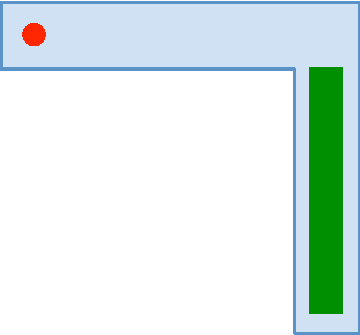
\includegraphics[width=.4\textwidth]{bar_counterex.pdf}
\caption{The Counterexample}
\label{fig:bar_counterex}
\end{figure}

To begin, let us consider the simplest possible space where a complex of sheaves has interesting behavior. Let $X=[0,1)$ with cell structure $v=\{0\}$ and $e=(0,1)$. A complex of sheaves over $X$ is completely described by two chain complexes and a chain map between them:
\[
\rho^{\bullet}_{e,v}:F^{\bullet}(v)\to F^{\bullet}(e)
\]
At first glance there should be a simple adaptation of Lemma~\ref{lem:chaincomplex_qis} to a pair of chain complexes. Indeed, we can use Theorem~\ref{thm:crawleyboevey} over each cell to obtain a candidate inclusion map from the cohomology sheaf into the complex:
\[
\xymatrix{F^i(v) \ar[r]^{\rho_{e,v}} & F^i(e) \\
B^i_v \oplus H^i_v \oplus B^{i-1}_v \ar[r]^{\rho_{e,v}} \ar[u]^{\cong}  & B^i_e \oplus H^i_e \oplus B^{i-1}_e \ar[u]_{\cong} \\
 H^i_v \ar[r]_{H^i(\rho)} \ar[u] & H^i_e \ar[u]}
\]
However such a map \emph{does not commute} in general and as such fails to define a sheaf map. For example, if $F^{\bullet}$ was the following pair of complexes and chain map
\[
\xymatrix{k \ar[r]^1 & k \\
0 \ar[r] \ar[u] & k \ar[u]_1}
\]
then the map $\rho$ takes the one and only generator of $H^i_v$ to an element of the boundaries $B^{i-1}_e$, which is non-zero, but zero in cohomology, since $H^i(\rho)=0$. We have provided a barcode version of this counter example in Figure~\ref{fig:bar_counterex}.


\subsection{Using the Calculus of Fractions Formulation}

In order to address the counterexample to the na\"ive approach, we will employ a zig-zag of morphisms. In this section we briefly review why such a zigzag is natural, when viewing the derived category as the \textbf{left calculus of fractions}~\cite{gabriel1967calculus}. An alternative description of the derived category goes as follows~\cite[p.52-3]{shepard}.

\begin{defn}[Derived Category via Fractions]\index{Derived@$D^b(\aat)$ derived category!calculus of fractions}\index{category!Derived@$D^b(\aat)$ derived category!calculus of fractions}
The \textbf{bounded derived category of cellular sheaves}, $D^b(\Shv(X))$, has the same collection of objects as $\Fun(X,\Ch(\Vect))$, but with a modified class of morphisms. A morphism from $F^{\bullet}$ to $G^{\bullet}$ is a diagram of the following form
\[
\xymatrix{ & J^{\bullet} & \\
F^{\bullet} \ar[ur] & & \ar[ul]_{\simeq} G^{\bullet}}
\]
where the arrow decorated with a $\simeq$ is a quasi-isomorphism. We declare two such morphisms (diagrams) to be the same if there is a larger, commutative diagram that fits in between them:
\[
\xymatrix{ & J_1^{\bullet} \ar[d]^{\simeq} & \\
F^{\bullet} \ar[ur] \ar[r] \ar[dr] & J_{12}^{\bullet} & \ar[l]_{\simeq} \ar[ul]_{\simeq} \ar[dl]^{\simeq} G^{\bullet} \\
& J_2^{\bullet} \ar[u]_{\simeq} & }
\]
\end{defn}

\subsection{The Equivalence}\label{subsec:graded_equivalence}

\begin{figure}
\centering
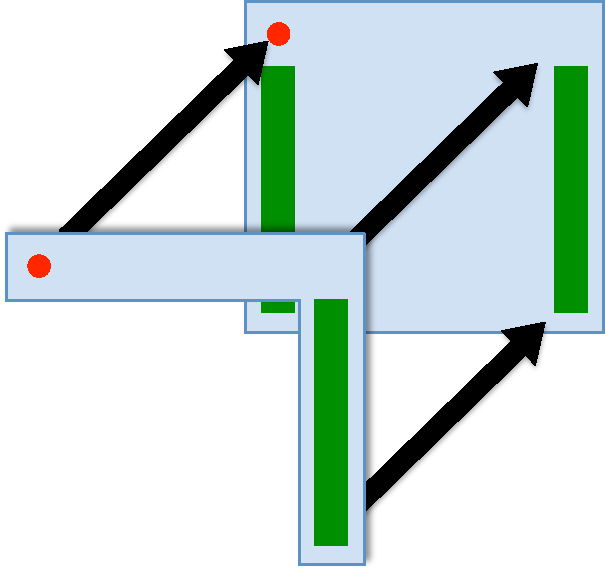
\includegraphics[width=.7\textwidth]{bar_replace.pdf}
\caption{Replacing the Counterexample with a Quasi-Isomorphic Sheaf}
\label{fig:bar_replace}
\end{figure}

We now proceed with a general method for addressing the earlier counterexample. The basic method of argument is that we will define a quasi-isomorphic complex of sheaves $J^{\bullet}$ where the na\"ive approach does work. This is visualized in Figure~\ref{fig:bar_replace}.
\[
\xymatrix{ & J^{\bullet} & \\
F^{\bullet} \ar[ur]^{\simeq} & & \ar[ul]_{\simeq} H^{*}F^{\bullet}}
\]

Let's first illustrate our method over the simple base space $X=[0,1)$.
\begin{lem}\label{lem:half-open-graded-equiv}\index{derived equivalence!with graded sheaves}\index{sheaf!cellular!derived equivalence with graded sheaves}
Over $X=[0,1)$ with cell structure $v=\{0\}$ and $e=(0,1)$, every bounded complex of cellular sheaves $F^{\bullet}$ is quasi-isomorphic to its graded cohomology sheaf $\cH^*F^{\bullet}$, i.e. $F^{\bullet}$ is \emph{isomorphic} to $\cH^*F^{\bullet}$ in the derived category.
\end{lem}
\begin{proof}
As before, we decompose the chain complex over the vertex $v$ and the edge $e$ so that $F^{\bullet}$ has the following form
\[
\xymatrix{ B^{i+1}_v\oplus H^{i+1}_v\oplus B^i_v \ar[r]^-{\rho_F^{i+1}} & B^{i+1}_e\oplus H^{i+1}_e\oplus B^i_e \\
B^{i}_v\oplus H^{i}_v\oplus B^{i-1}_v \ar[r]^-{\rho_F^{i}} \ar[u]^{d^i_v} & B^{i}_e\oplus H^{i}_e\oplus B^{i-1}_e \ar[u]_{d^i_e}
}
\]
The map $\rho^i_F$ has an easily described form in this basis.
\[
\rho^i_F=
\left[
\begin{array}{ccc}
\alpha^i & 0 & 0 \\
\gamma^i & H^i\rho & 0 \\
\delta^i & \beta^{i-1} & \alpha^{i-1}
\end{array}
\right]
\]
The na\"ive inclusion map's failure to commute is precisely described by non-zero terms in the submatrix $\beta^{i-1}$, as can be seen by inspecting the diagram below.
\[
\xymatrix{
B^i_v \oplus H^i_v \oplus B^{i-1}_v \ar[r]^-{\rho^i_F}  & B^i_e \oplus H^i_e \oplus B^{i-1}_e  \\
 H^i_v \ar[r]_-{H^i(\rho)} \ar[u] & H^i_e \ar[u]
 }
\]
However, the complex of sheaves $F^{\bullet}$ is quasi-isomorphic to the complex $J^{\bullet}$ defined as follows.
\[
\xymatrix{ B^{i+1}_v\oplus B^{i+1}_e \oplus H^{i+1}_v\oplus B^i_v \oplus B^{i}_e \ar[r]^-{\rho_J^{i+1}} & B^{i+1}_e\oplus H^{i+1}_e\oplus B^i_e \\
B^{i}_v\oplus B^{i}_e\oplus H^{i}_v\oplus B^{i-1}_v \oplus B^{i-1}_e \ar[r]^-{\rho^{i}_J} \ar[u]^{d^i_v} & B^{i}_e\oplus H^{i}_e\oplus B^{i-1}_e \ar[u]_{d^i_e}
}
\]
The matrix representation for $\rho^i_J$ has the desired form:
\[
\rho^i_J=
\left[
\begin{array}{ccccc}
0 & \id & 0 & 0 & 0\\
 \gamma^i & 0 & H^i\rho & 0 & 0 \\
\delta^i & 0 & 0 & & \id
\end{array}
\right]
\]
The quasi-isomorphism $q^{\bullet}:F^{\bullet}\to J^{\bullet}$ is defined over the vertex $v$ in any given degree $i$ as
\[
q^i_v=
\left[
\begin{array}{ccc}
\id & 0 & 0 \\
\alpha^i & 0 & 0 \\
0 & \id & 0 \\
0 & 0 & \id \\
0 & \beta^{i-1} & \alpha^{i-1} 
\end{array}
\right]
\]
and over the edge $e$ as $q^i_e=\id$. By construction, the complex $J^{\bullet}$ has a well defined sheaf map
\[
\xymatrix{
B^{i}_v\oplus B^{i}_e\oplus H^{i}_v\oplus B^{i-1}_v \oplus B^{i-1}_e \ar[r]^-{\rho^{i}_J}  & B^{i}_e\oplus H^{i}_e\oplus B^{i-1}_e \\
H^{i}_v \ar[r]_-{H^i\rho} \ar[u] & H^i_e \ar[u]
}
\]
which extends to a quasi-isomorphism $\iota:\cH^{*}F^{\bullet}\hookrightarrow J^{\bullet}$ since each of the differentials $\cH^iF^{\bullet}\to \cH^{i+1}F^{\bullet}$ are zero. This completes the proof.
\end{proof}

We can now prove the general theorem of interest.

\begin{thm}\label{thm:1D-graded-equiv}\index{derived equivalence!with graded sheaves}\index{sheaf!cellular!derived equivalence with graded sheaves}
Let $X$ be an arbitrary one dimensional cell complex and $F^{\bullet}$ a complex of sheaves over $X$. Then $F^{\bullet}$ is quasi-isomorphic to its graded cohomology sheaf. In particular, we have the equivalence of categories
\[
D^b(\Shv(X))\simeq \Shv(X;\grVect).
\]
\end{thm}
\begin{proof}
The bulk of the argument is contained in Lemma~\ref{lem:half-open-graded-equiv}, which we show extends to the desired generality. The definition of $J^i(v)$ where $v$ is a vertex with more than one incident edge is easily modified as follows:
\[
J^i(v):=B^i_v\bigoplus_{e\geq v} B^i_e \oplus H^i_v \oplus B^{i-1}_v
 \bigoplus_{e\geq v} B^{i-1}_e
\]
The restriction map to a single edge $e'$ is defined exactly as in Lemma~\ref{lem:half-open-graded-equiv} with the stipulation that factors $B^i_e$ and $B^{i-1}_e$ where $e\neq e'$ are mapped to zero.

This argument implies that we can define the desired morphism 
\[
\xymatrix{ & J^{\bullet} & \\
F^{\bullet} \ar[ur]_q^{\simeq} & & \ar[ul]_{\simeq}^{\iota} H^{*}F^{\bullet} }
\]
in an open neighborhood of a vertex. However, since over each edge $q^i_{e}:F^i(e)\to J^i(e)$ is defined to be the identity map, these locally defined maps agree on the edges and hence give a globally defined map of sheaves. This shows the equivalence with the graded cohomology sheaf.

One can check that every map of sheaves $f:F^{\bullet}\to G^{\bullet}$ extends to a map of the associated sheaves $J_f:J^{\bullet}_F\to J^{\bullet}_G$ so the construction is functorial and hence defines an equivalence of categories.
\end{proof}
